%%%%%%%%%%%%%%%%%%%%%%%%%%%%%%%%%%%%% 
%% LE2I beamer template
%% Guillaume Lemaitre, October 2014
%%%%%%%%%%%%%%%%%%%%%%%%%%%%%%%%%%%%% 

\documentclass[table]{beamer}

\usepackage[utf8]{inputenc}
\usepackage[T1]{fontenc} 
\usetheme{le2i} 

%% The amssymb package provides various useful mathematical symbols
\usepackage{amssymb}
%% The amsthm package provides extended theorem environments
\usepackage{amsthm}
%% amsmath for math environment
\usepackage{amsmath}

\DeclareMathOperator*{\argmin}{arg\,min}
\DeclareMathOperator*{\argmax}{arg\,max}
\DeclareMathOperator*{\sign}{sign}

%% figure package
\usepackage{epsf,graphicx}
\usepackage{epstopdf}
\usepackage{subfigure}
\usepackage{transparent}
\usepackage{fixltx2e}

%% In order to draw some graphs
\usepackage{tikz,xifthen}
\usepackage{tikz-qtree}
\usepackage{adjustbox}
\usetikzlibrary{decorations.pathmorphing}
\usetikzlibrary{fit}
\usetikzlibrary{backgrounds}
\usetikzlibrary{shapes,arrows,shadows}
\usetikzlibrary{calc,decorations.pathreplacing,decorations.markings,positioning}
\usetikzlibrary{snakes,decorations.text,shapes,patterns}
% \usepackage{scalefnt,lmodern,booktabs}

\usepackage{mathtools}

%% Package for cross and tick symbols
\usepackage{pifont}
\newcommand{\tick}{\color{green!60!black!80}\ding{51}}
\newcommand{\cross}{\color{red!60!black!80}\ding{55}}

%\usepackage[table]{xcolor}

\title{Introduction to Image Processing}
\author{Guillaume Lema\^itre \\ \texttt{guillaume.lemaitre@udg.edu}}
\date{Lecture 2\\ 21\textsuperscript{st} Sept. 2015}

\institute{Universit\'e de Bourgogne} 

%% Uncomment if you want to avoid thousand of bullet inside the menu
% \usepackage{etoolbox}
% \makeatletter
% \patchcmd{\slideentry}{\advance\beamer@xpos by1\relax}{}{}{}
% \def\beamer@subsectionentry#1#2#3#4#5{\advance\beamer@xpos by1\relax}%
% \makeatother

\begin{document}

% Show the title page
\begin{frame}
  \titlepage
\end{frame}

% Show the table of contents
\begin{frame}
  \tableofcontents[sectionstyle=show,subsectionstyle=show,subsubsectionstyle=hide]
\end{frame}

\section{Intensity Transformation}

\subsection{Foreword}

\begin{frame}
  \frametitle{Intensity Transformation}
  \framesubtitle{Foreword}
  \begin{block}{Definition}\footnotesize
    \begin{equation}
      g(x,y) = T[f(x, y)]
    \end{equation}In this part, $g$ depends \emph{only} on the value of $f$ at a single point $(x,y)$
    \begin{equation}
      s = T[r]
    \end{equation}
    \begin{figure}
      \centering
      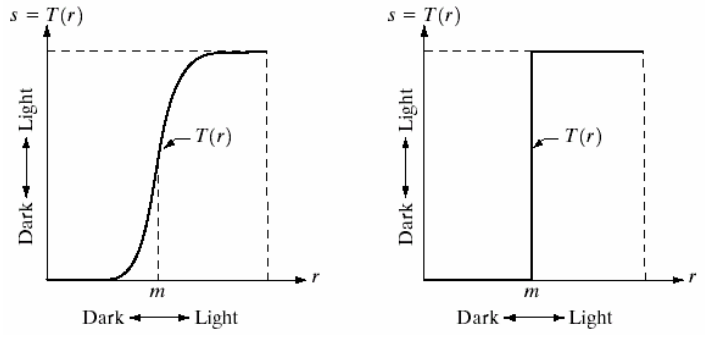
\includegraphics[height=.4\textheight]{./images/cont_stretch.png}
    \end{figure}
  \end{block}
\end{frame}

\begin{frame}
  \frametitle{Intensity Transformation}
  \framesubtitle{Foreword}
  \begin{block}{Gray-scale transform}\footnotesize
    \begin{figure}
      \centering
      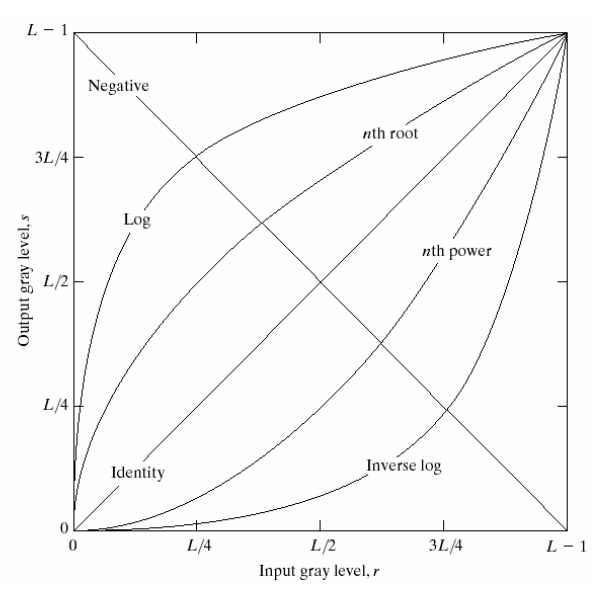
\includegraphics[height=.6\textheight]{./images/gray_trans.png}
    \end{figure}
  \end{block}
\end{frame}

\subsection{Basic transformation}

\begin{frame}
  \frametitle{Intensity Transformation}
  \framesubtitle{Basic transformations}
  \begin{block}{Gray-scale transform}\footnotesize
    \begin{itemize}
    \item Image negatives
    \item Log transformations
    \item Power-law (Gamma) Transformations
    \item Contrast stretching - Intensity-level slicing
    \item Bit-plane slicing
    \item[$\rightarrow$] Check the Ipython notebook
    \end{itemize}
  \end{block}
\end{frame}

\subsection{Histogram Equalization}

\begin{frame}
  \frametitle{Intensity Transformation}
  \framesubtitle{Histogram equalization}
  \begin{block}{Principle}\footnotesize
    \begin{figure}
      \centering
      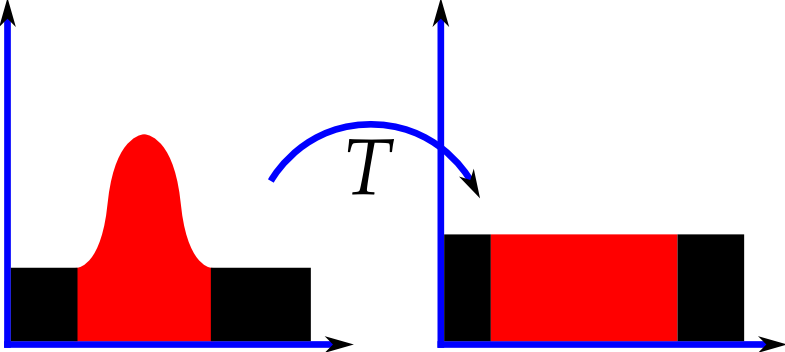
\includegraphics[width=.7\textwidth]{./images/histogram-equalization.png}
    \end{figure}
    \begin{itemize}
      \item Equally make use of all the available gray levels in the dynamic range
    \end{itemize}
  \end{block}
\end{frame}

\begin{frame}
  \frametitle{Intensity Transformation}
  \framesubtitle{Histogram equalization}
  \begin{block}{Formulation}\footnotesize
    \begin{itemize}
      \item Find the gray level mapping $y = f(x)$
      \item All pixels in $dx$ will be mapped into $dy$ 
        \begin{equation}\label{eq:eq1}
          p(y)dy=p(x)dx \ .
        \end{equation}
    \end{itemize}
    \begin{figure}
      \centering
      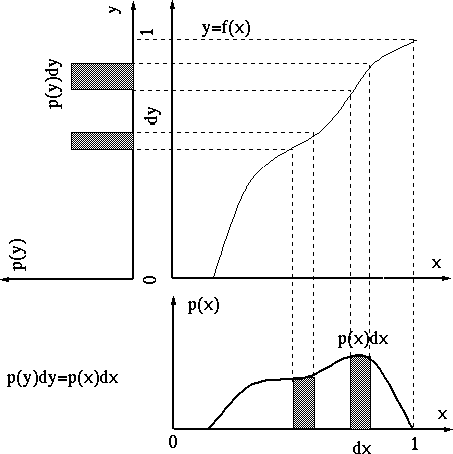
\includegraphics[width=.3\textwidth]{./images/histogram-equalization2.png}
    \end{figure}
  \end{block}
\end{frame}

\begin{frame}
  \frametitle{Intensity Transformation}
  \framesubtitle{Histogram equalization}
  \begin{block}{Formulation}\footnotesize
    \begin{itemize}
      \item Equalizing is equivalent to force $p(y)=1$ so that
        \begin{equation}\label{eq:eq2}
          \int_{0}^{1} p(x)dx = \int_{0}^{1} dy = 1 \ ,
        \end{equation}
        \begin{equation}\label{eq:eq3}
          p(x)dx = dy \text{ or } p(x)=\frac{dy}{dx} \ ,
        \end{equation}
      \item By integrating both sides
        \begin{equation}\label{eq:eq4}
          y = f(x) = \int_{0}^{x} p(u)du = P(x) - P(0) = P(x) \ ,
        \end{equation}
    \end{itemize}
  \end{block}
\end{frame}

\begin{frame}
  \frametitle{Intensity Transformation}
  \framesubtitle{Histogram equalization}
  \begin{block}{Intuitive aspects}\footnotesize
    \begin{itemize}
      \item If $p(x)$ is low, $P(x)$ shallow slope, $dy$ will be narrow, causing $p(y)$ to be high
      \item If $p(x)$ is high, $P(x)$ steep slope, $dy$ will be wide, causing $p(y)$ to be low
    \end{itemize}
  \end{block}
\end{frame}

\begin{frame}
  \frametitle{Intensity Transformation}
  \framesubtitle{Histogram equalization}
  \begin{block}{Exercise}\footnotesize
    \begin{center}
      \renewcommand{\arraystretch}{1.5}
      \begin{tabular}{|ccc|}\hline
        \rowcolor{gray!20}
        $r_k$ & $n_k$ & $p_r(r_k) = \frac{n_k}{MN}$ \\ \hline
        $r_0 = 0$ & $790$ & $0.19$ \\
        $r_1 = 1$ & $1023$ & $0.25$ \\
        $r_2 = 2$ & $850$ & $0.21$ \\
        $r_3 = 3$ & $656$ & $0.16$ \\
        $r_4 = 4$ & $329$ & $0.08$ \\
        $r_5 = 5$ & $245$ & $0.06$ \\
        $r_6 = 6$ & $122$ & $0.03$ \\
        $r_7 = 7$ & $81$  & $0.02$ \\ \hline
      \end{tabular}
    \end{center}
  \end{block}
\end{frame}

\subsection{Histogram specification - matching}

\begin{frame}
  \frametitle{Intensity Transformation}
  \framesubtitle{Histogram specification matching}
  \begin{block}{Principle}\footnotesize
    \begin{itemize}
    \item Similar to histogram equalization
    \item Involve an extra step to match a given histogram instead of a uniform histogram
    \end{itemize}
  \end{block}
  \begin{block}{Algorithm}\footnotesize
    \begin{itemize}
    \item Perform histogram equalization to find $s = T(r)$
    \item Perform histogram equalization to find $s = G(z)$
    \item Find the inverse transform $z = G^{-1}(s)$
    \item Apply the successive mapping $r \xRightarrow{T(\cdot)} s \xRightarrow{G^{-1}(\cdot)} z$
    \end{itemize}
  \end{block}
\end{frame}

\begin{frame}
  \frametitle{Intensity Transformation}
  \framesubtitle{Histogram specification matching}
  \begin{block}{Exercise}\footnotesize
    \begin{center}
      \renewcommand{\arraystretch}{1.5}
      \begin{tabular}{|cc|}\hline
        \rowcolor{gray!20}
        $z_k$ & $p_z(z_k) = \frac{n_k}{MN}$ \\ \hline
        $z_0 = 0$ & $0.00$ \\
        $z_1 = 1$ & $0.00$ \\
        $z_2 = 2$ & $0.00$ \\
        $z_3 = 3$ & $0.15$ \\
        $z_4 = 4$ & $0.20$ \\
        $z_5 = 5$ & $0.30$ \\
        $z_6 = 6$ & $0.20$ \\
        $z_7 = 7$ & $0.15$ \\ \hline
      \end{tabular}
    \end{center}
  \end{block}
\end{frame}

\subsection{From global to local}

\begin{frame}
  \frametitle{Intensity Transformation}
  \framesubtitle{From global to local}
  \begin{block}{Local enhancement}\footnotesize
    \begin{itemize}
      \item Define a square neighbourhood
      \item Move pixel to pixel
      \item Apply any processing
        \begin{figure}
          \centering
          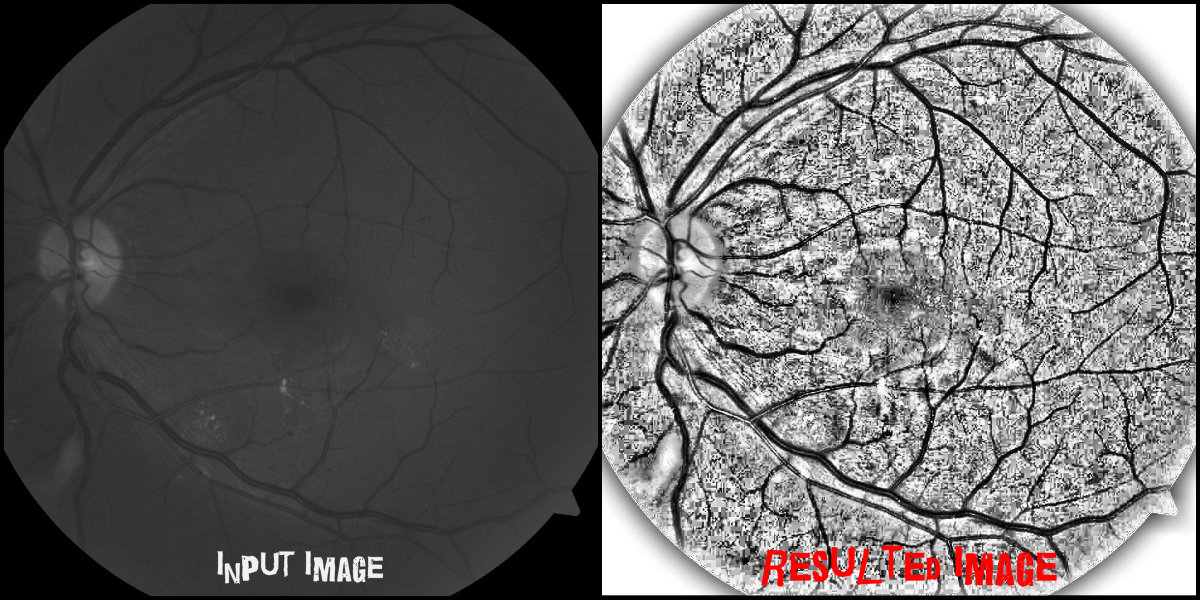
\includegraphics[width=.8\textwidth]{./images/local-histogram-equalization.jpg}
        \end{figure}
      \end{itemize}
  \end{block}
\end{frame}

%---------------------
\section{Spatial Filtering}

\subsection{Preface}

\begin{frame}
  \frametitle{Spatial Filtering}
  \framesubtitle{Preface}
  \begin{block}{How-to}
    \begin{itemize}
    \item Use of spatial masks for image processing 
    \item Linear and Nonlinear 
    \end{itemize}
  \end{block}
  \begin{block}{Different types}
    \begin{itemize}
    \item Low-pass filters 
    \item High-pass filters 
    \item Band-pass filters
    \end{itemize}
  \end{block}
\end{frame}

%------------
\begin{frame}
\frametitle{Spatial Filtering}
\begin{itemize}
  \item \textbf{Low-pass} filters eliminate or attenuate high frequency component ({\color{blue} sharp image details}) in the frequency domain, and result in image {\color{blue} blurring}.
    \item \textbf{High-pass} filters eliminate and attenuate the low frequency components and result in {\color{blue} sharpening edges} and other sharp details. 
      \item \textbf{Band-pass} filters remove or select a frequency region between low and high frequencies. 
\end{itemize}
\end{frame}
%----------
\subsection{Linear filtering}
\begin{frame}
\frametitle{Spatial Filtering}
\framesubtitle{Linear filtering}
\begin{center}
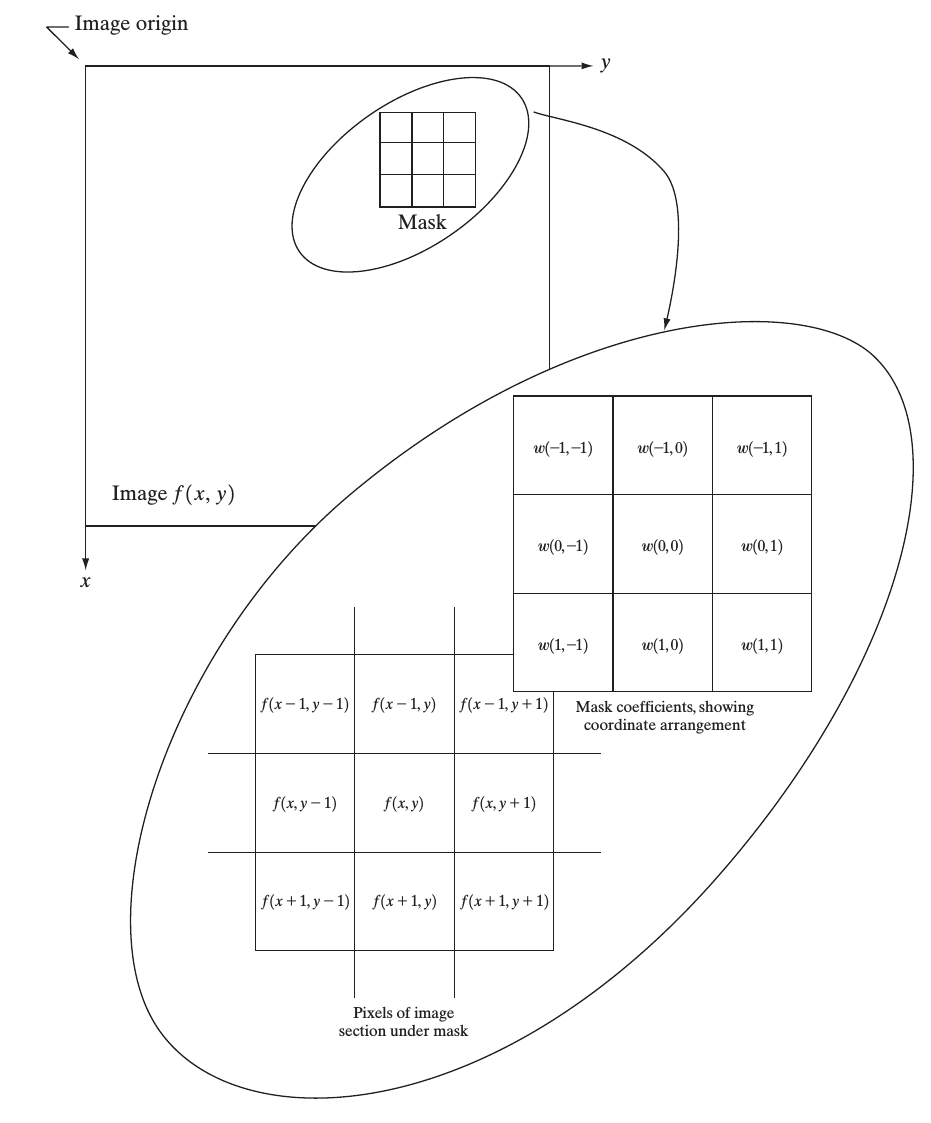
\includegraphics[scale=0.23]{images/Spatial2.png}
\end{center}
\end{frame}

\begin{frame}
\frametitle{Spatial Filtering}
\framesubtitle{Linear filtering}
\begin{block}{Correlation}
\begin{equation}
  g(x,y) = \sum^{a}_{s=-a}\sum^{b}_{t=-b} w(s,t)f(x+s, y+t)
\end{equation}
\end{block}
\begin{block}{Convolution}
\begin{equation}
  g(x,y) = \sum^{a}_{s=-a}\sum^{b}_{t=-b} w(s,t)f(x-s, y-t)
\end{equation}
\end{block}
\end{frame}

\begin{frame}
  \frametitle{Spatial Filtering}
  \framesubtitle{Linear filtering}
  \begin{block}{Computation example}
    \begin{columns}
      \begin{column}{.5\linewidth}
        \begin{center}
          \begin{tabular}{|ccccc|}\hline
            0 & 0 & 0 & 0 & 0\\ 
            0 & 0 & 0 & 0 & 0\\ 
            0 & 0 & 1 & 0 & 0\\ 
            0 & 0 & 0 & 0 & 0\\ 
            0 & 0 & 0 & 0 & 0\\\hline 
          \end{tabular}
        \end{center}
      \end{column}
       \begin{column}{.5\linewidth}
        \begin{center}
          \begin{tabular}{|ccc|}\hline
            1 & 2 & 3 \\ 
            4 & 5 & 6 \\ 
            7 & 8 & 9 \\ \hline
          \end{tabular}
        \end{center}
      \end{column}
    \end{columns}
  \end{block}
\end{frame}



\begin{frame}
\frametitle{Spatial filter}
\framesubtitle{Linear filtering}
\begin{block}{Vector representation}
The basic approach is to sum products between the mask coefficients and the intensities of the pixels under the mask at a specific location in the image. \\
For $3 \times 3$ filter: 
$$R = w_{1}z_{1}+w_{2}z_{2}+...+w_{9}z_{9}$$
\end{block}
\end{frame}
%-----------

\subsection{Smoothing linear filtering}

\begin{frame}
\frametitle{Spatial Filtering}
\framesubtitle{Smoothing linear filter}
\begin{itemize}
\item  Replacing the value of every pixel in an image by the average of the gray levels in the neighborhood defined by the filter mask.
\item Averaging filter 
\item {\color{red} Blurring the edges}
\item Two $3\times 3$ smoothing (averaging) filter masks. The constant multiplier in front of each mask is equal to the sum of the values of its coefficients, as is required to compute an average.
\begin{center}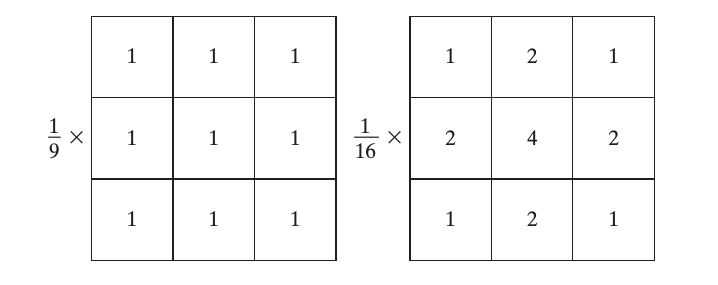
\includegraphics[scale=0.4]{images/Spatial3.png}\end{center}
\end{itemize}
\end{frame}
%-----------
\begin{frame}
\frametitle{Spatial Filtering}
\framesubtitle{Smoothing linear filter}
Results of smoothing with square averaging filter masks of sizes $n=\{3, 5, 9, 15, 35\}$
\begin{center}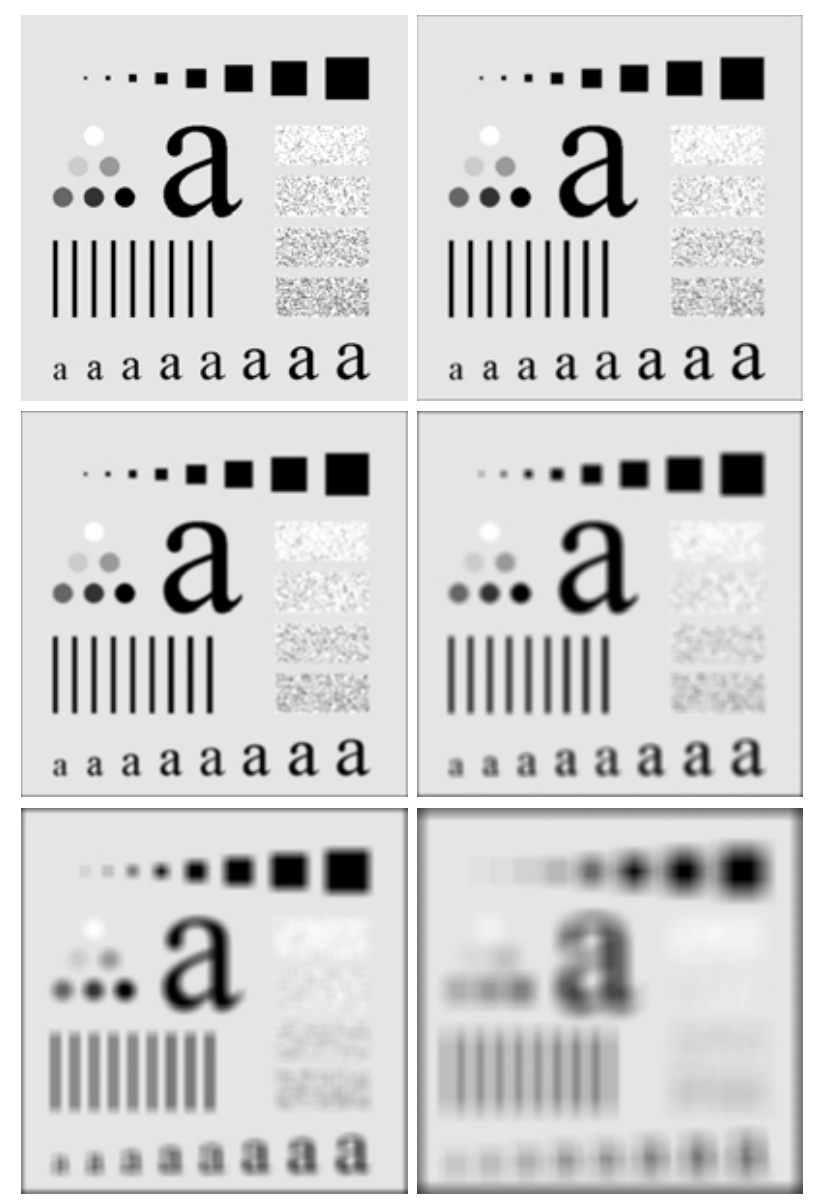
\includegraphics[scale=0.19]{images/Spatial4-averagefilter.png}\end{center}
\end{frame}

%----------
\begin{frame}
\frametitle{Spatial Filtering}
\framesubtitle{Smoothing linear filter} 
\begin{center}
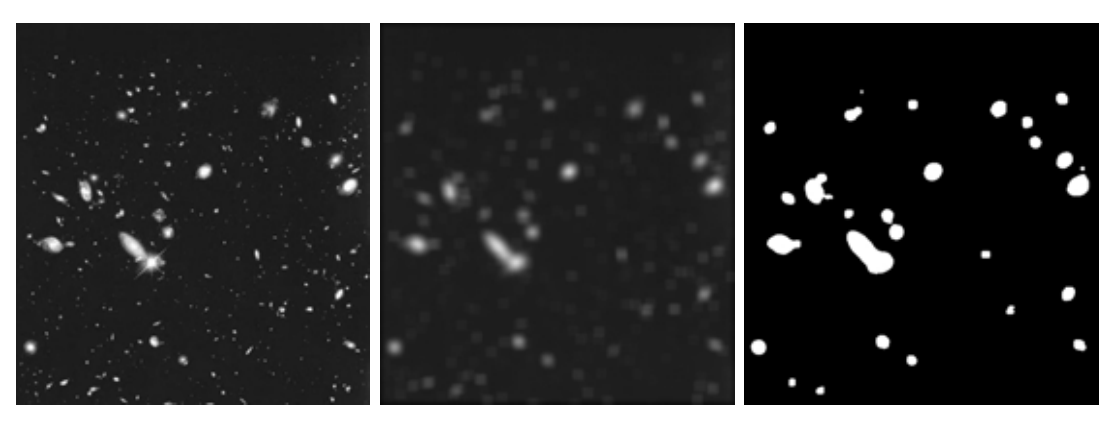
\includegraphics[scale=0.3]{images/Spatial5-averagefilter.png}
\end{center}
\end{frame}
%-----------

\subsection{Smoothing non-linear filtering}

\begin{frame}
\frametitle{Spatial Filtering}
\framesubtitle{Smoothing non-linear filter}
Median filtering also used for noise elimination. 
\begin{itemize}
\item The gray level of each pixel is replaced by the median gray levels in the neighborhood of the pixel instead of the average.
\item X-ray image of the circuit board corrupted by salt-and-pepper noise. Noise reduction with $3 \times 3$ average and median filter, respectively.
\item[]\begin{center}
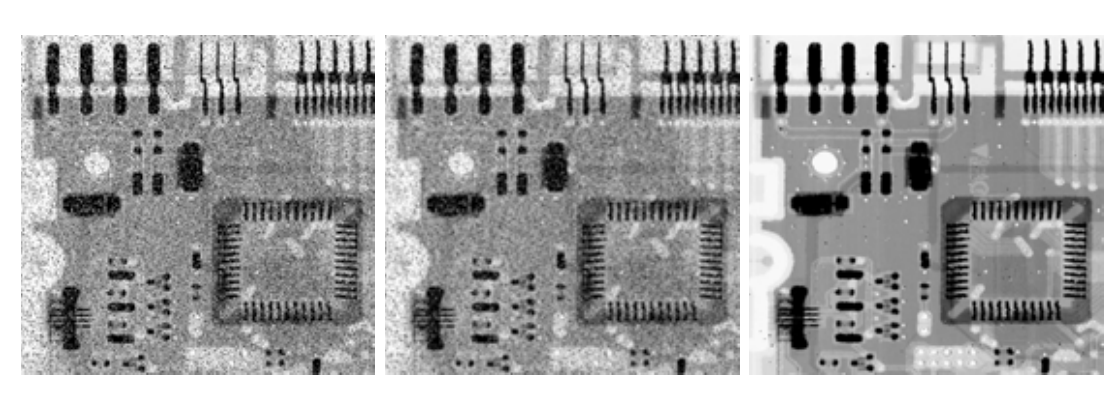
\includegraphics[scale=0.3]{images/Spatial6-averagemedian.png}
\end{center}  
\end{itemize}
\end{frame}
%---------

\subsection{Sharpening filter}

\begin{frame}
\frametitle{Spatial Filtering}
\framesubtitle{Sharpening filter}
\begin{block}{Aim}
\begin{itemize}
\item[$\rightarrow$] To highlight fine detail or to enhance blurred detail. 
\begin{itemize}
\item smoothing $\approx$ integration
\item sharpening $\approx$ differentiation
\end{itemize}
\end{itemize}
\end{block}
\begin{block}{Categories of sharpening filters}
\begin{itemize}
\item Derivative operator 
\item Basic high-pass spatial filter 
\item High-boost filtering 
\end{itemize}
\end{block}
\end{frame}
%------------
\begin{frame}
\frametitle{Spatial Filtering}
\framesubtitle{Sharpening filter - Derivative filter}
\begin{block}{First-order derivative}
$$\frac{\partial f}{\partial x} = f(x+1) - f(x)$$
\end{block}
\begin{block}{Second-order derivative}
$$\frac{\partial^{2}f}{\partial x^{2}} = f(x+1)+f(x-1) - 2f(x)$$
\end{block}
\end{frame}
%-----------
\begin{frame}
\frametitle{Spatial Filtering}
\framesubtitle{Sharpening filter - Derivative filter}
\begin{center}
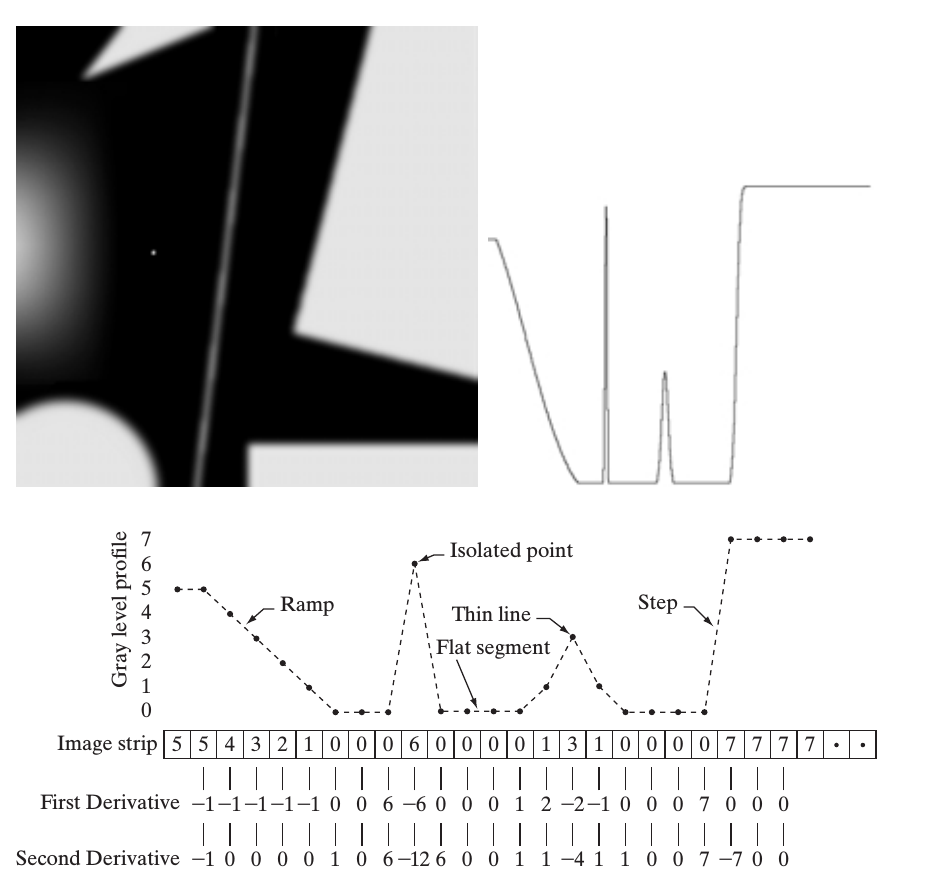
\includegraphics[scale=0.3]{images/Spatial7-derivative.png}
\end{center}
\end{frame}
%-----------
\begin{frame}
  \frametitle{Spatial Filtering}
  \framesubtitle{Sharpening filter - Derivative filter}
  \begin{block}{First-order derivative}
    \begin{itemize}
    \item 0 in constant gray segments
    \item Non-zero at the onset of steps or ramps
    \item Non-zero along ramps
    \end{itemize}

  \end{block}
  \begin{block}{Second-order derivative}
    \begin{itemize}
    \item 0 in constant gray segments
    \item Non-zero at the onset and end of steps or ramps
    \item 0 along ramps of constant slope.
    \end{itemize}

  \end{block}
\end{frame}
%-----------
\begin{frame}
\frametitle{Spatial Filtering}
\framesubtitle{Sharpening filter - Derivative filter}
  \begin{block}{First-order derivative}
    \begin{itemize}
    \item produce thicker edges in an image
    \item have a stronger response to a gray-level step
    \end{itemize}
  \end{block}
  \begin{block}{Second-order derivative}
    \begin{itemize}
    \item have a stronger response to fine detail, such as thin lines and isolated points
    \item produce a double response at step changes in gray level
    \item have stronger response to a line than to a step and to a point than to a line
    \end{itemize}
  \end{block}
\end{frame}
%-----------
% \begin{frame}
% \frametitle{Spatial Filtering}
% \framesubtitle{Sharpening filter - Basic Highpass Spatial filter}
% \begin{itemize}
% \item Cross section of frequency domain filter:
% \begin{center}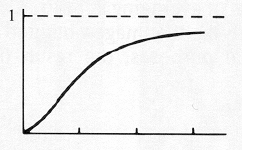
\includegraphics[scale=0.5]{images/HPS-f.png}\end{center} 
% \item Cross section of spatial domain filter:
% \begin{center}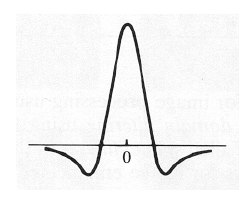
\includegraphics[scale=0.5]{images/HPS-S.png}\end{center} 
% \end{itemize}
% \end{frame}
%-----------
% \begin{frame}
% \frametitle{Spatial Filtering}
% \framesubtitle{Sharpening filter - Basic Highpass Spatial filter}
% \begin{itemize}
% \item The filter should have positive coefficients near the center and negative in the outer periphery
% \begin{center}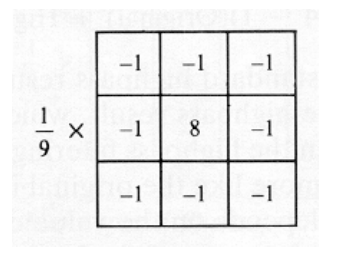
\includegraphics[scale=0.3]{images/HPF.png}\end{center}
% \item The sum of the coefficients is 0, indicating that when the filter is passing over regions of almost stable gray levels, the output of the mask is 0 or very small.
% \item Some scaling and/or clipping is involved to compensate for possible negative gray levels after filtering.
% \end{itemize}
% \end{frame}
%-----------
\begin{frame}
\frametitle{Spatial Filtering}
\framesubtitle{Sharpening filter - 2D, Second order derivatives}
\begin{itemize}
\item Isotropic filters, rotation invariant 
\item Laplacian (linear operator)
$$\triangledown^2 f = \frac{\partial^2 f}{\partial x^2}+ \frac{\partial^2 f}{\partial y^2}$$
\item Discrete version: 
$$\frac{\partial^2 f}{\partial x^2} = f(x+1,y) + f(x-1,y) -2f(x,y)$$
$$\frac{\partial^2 f}{\partial y^2} = f(x,y+1) + f(x,y-1) -2f(x,y)$$ 
\end{itemize}
\end{frame}
%-----------
\begin{frame}
\frametitle{Spatial Filtering}
\framesubtitle{Sharpening filter - 2D, Second order derivative}
\begin{itemize}
\item Digital implementation 
$$\triangledown^2 f = [f(x+1,y)+f(x-1,y)+f(x,y+1)+f(x,y-1)]-4f(x,y)$$
\item Two definitions, one is negative of the other
\[ g(x,y) =
  \begin{cases}
    f(x,y)-\triangledown^2 f(x,y)  & \quad \text{Center of the mask is negative} \\
    f(x,y)+\triangledown^2 f(x,y)  & \quad \text{Center of the mask is positive} \\
  \end{cases}
\]
\end{itemize}
\end{frame}
%----------
\begin{frame}
\frametitle{Spatial Filtering}
\framesubtitle{Sharpening filter - 2D, Second order derivative}
\begin{itemize}
\item Filtering and recovering the original part: 
\scriptsize{
$$ g(x,y) = f(x,y) - [f(x+1,y)+f(x-1,y)+f(x,y+1)+f(x,y-1)]+4f(x,y)$$
$$ g(x,y) = 5f(x,y) - [f(x+1,y)+f(x-1,y)+f(x,y+1)+f(x,y-1)]$$
}
\end{itemize}
\end{frame}
%----------
\begin{frame}
\frametitle{Spatial Filtering}
\framesubtitle{Sharpening filter - 2D, Second order derivative}
\begin{center}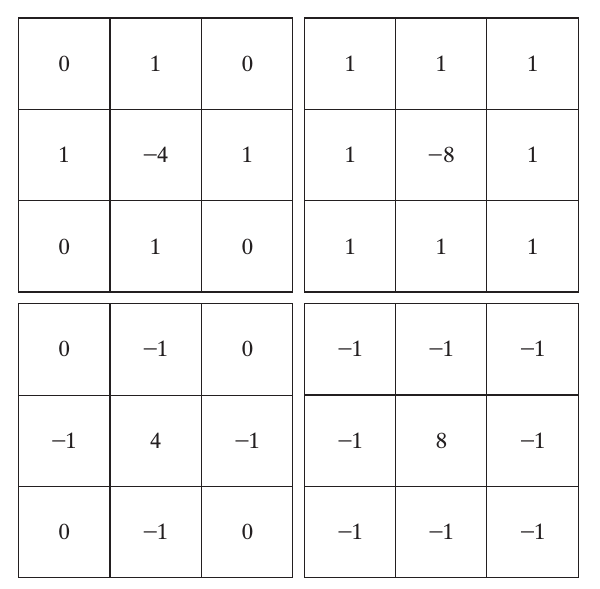
\includegraphics[scale=0.3]{images/Spatial7-laplacian.png}\end{center}
\end{frame}
%---------
\begin{frame}
\frametitle{Spatial Filtering}
\framesubtitle{Sharpening filter - 2D, Second order derivative}
Image of the north pole of the moon, laplacian filtered image, laplacian image scaled for display and image enhanced by laplacian, respectively.
\begin{center}
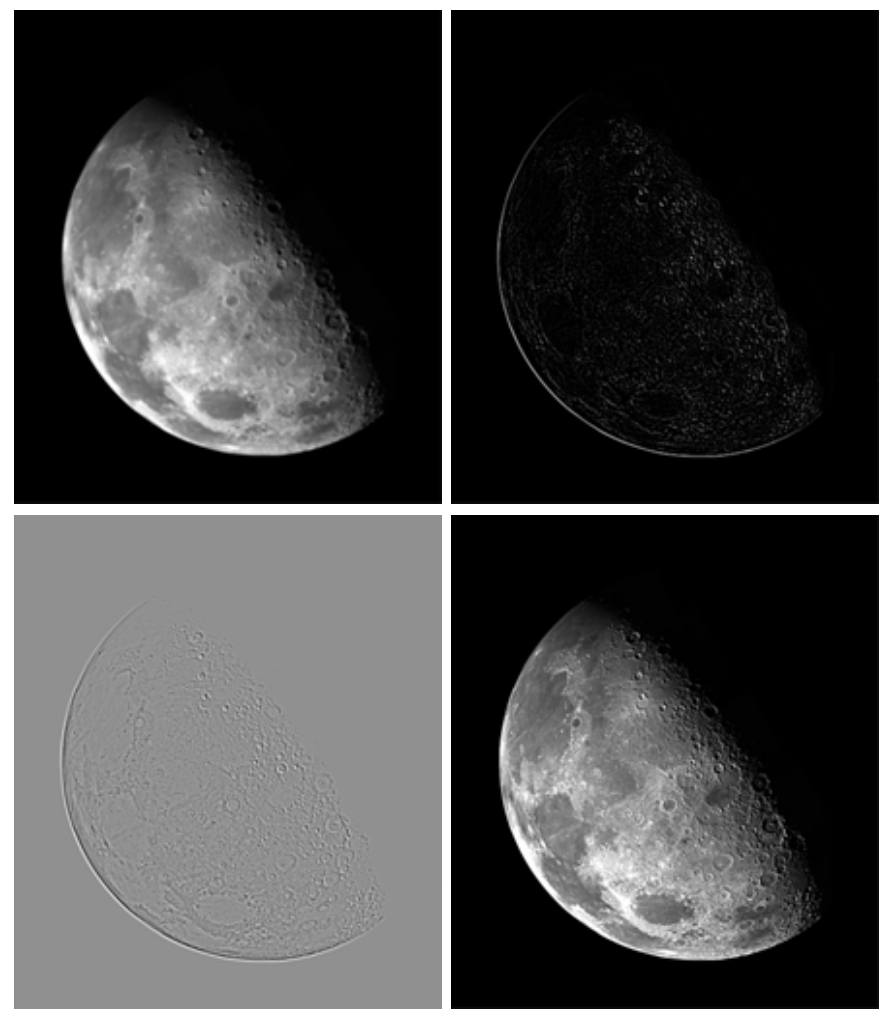
\includegraphics[width = 0.45\textwidth, height = 0.6\textheight]{images/Spatial8-laplacian-ex.png} 
\end{center}
\end{frame}
%-----------
\begin{frame}
\frametitle{Spatial Filtering}
\framesubtitle{Sharpening filter}

\begin{block}{High-boost filter}
\begin{enumerate}
\item Blur the image (low-pass filtering)
\item Subtract the blurred image from the original (high frequency image)
\item Add the previous mask 
\end{enumerate}
\begin{itemize}
\item $k =1$ --> Unsharp masking 
\item $k >1$ --> Highboost filtering
\end{itemize}
\end{block}
\end{frame}
% %-----------
% \begin{frame}
% \framesubtitle{Spatial Filtering}
% \framesubtitle{Sharpening filter - High-boost filter}
% \begin{center}
% 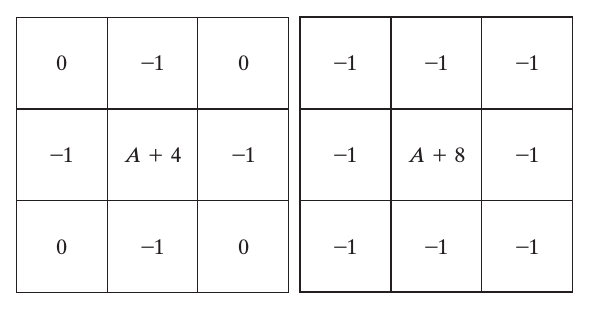
\includegraphics[scale=0.3]{images/Spatial9-HBF.png}
% \end{center}
% \end{frame}
%-----------
\begin{frame}
\frametitle{Spatial Filtering}
\framesubtitle{Gradient filter - first derivative}
\begin{itemize}
\item The most common method of differentiation in image processing
 $$\triangledown f = 
\begin{bmatrix}
G_x\\G_y
\end{bmatrix} = 
\begin{bmatrix}
\frac{\partial f}{\partial x}\\
 \frac{\partial f}{\partial y}
 \end{bmatrix}
$$
\item It is non-isotropic
\item Its magnitude (often call the gradient) is rotation invariant
$$\triangledown f = \vert G_{x} \vert + \vert G_{y} \vert = [(\frac{\partial f}{\partial x})^2 + (\frac{\partial f}{\partial x})^2]^{1/2} $$
\end{itemize}

\end{frame}
%-----------
\begin{frame}
\frametitle{Spatial Filtering}
\framesubtitle{Gradient filter - first derivative}
Different masks use to calculate the gradient of a region of interest with $z_{5}$ as a central pixel, Robert cross gradient masks middle row and  Sobel filters in the last row.
\begin{center}
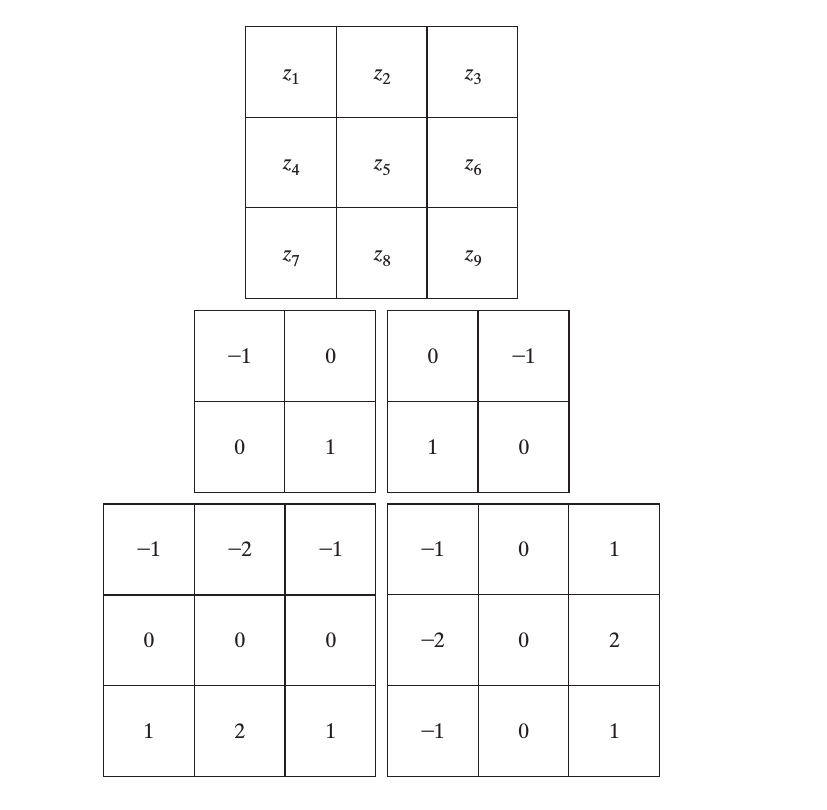
\includegraphics[scale=0.26]{images/Spatial10-gradient.png}
\end{center}
\end{frame}
%----------
\begin{frame}
\frametitle{Spatial Filtering}
\framesubtitle{Gradient filter - first derivative}
\begin{itemize}
\item Computation:
\item Cross differences as used in early development of digital image processing: 
$G_x = (z_9 - z_5)$, \quad $ G_y = (z_8 - z_6)$
\item Robert cross gradient: 
$$ \triangledown f \approx [(z_9 - z_5)^2 + (z_8 - z_6)^2]^{1/2}$$
\item Sobel filter 
\scriptsize{
$$ \triangledown f \approx \vert (z_7 + 2 z_8 + z_9) - (z_1 + 2 z_2 + z_3) \vert + \vert (z_3 + 2 z_9 + z_6) - (z_1 + 2 z_4 + z_7) \vert$$
}
\end{itemize}

\end{frame}

% %----------
% \begin{frame}
% \frametitle{Spatial Filtering}
% Whole body bone scane, laplacian image, sharpened image using the laplacian and sobel filtered image, respectively from right to left and first row to second. 
% \begin{center}
% 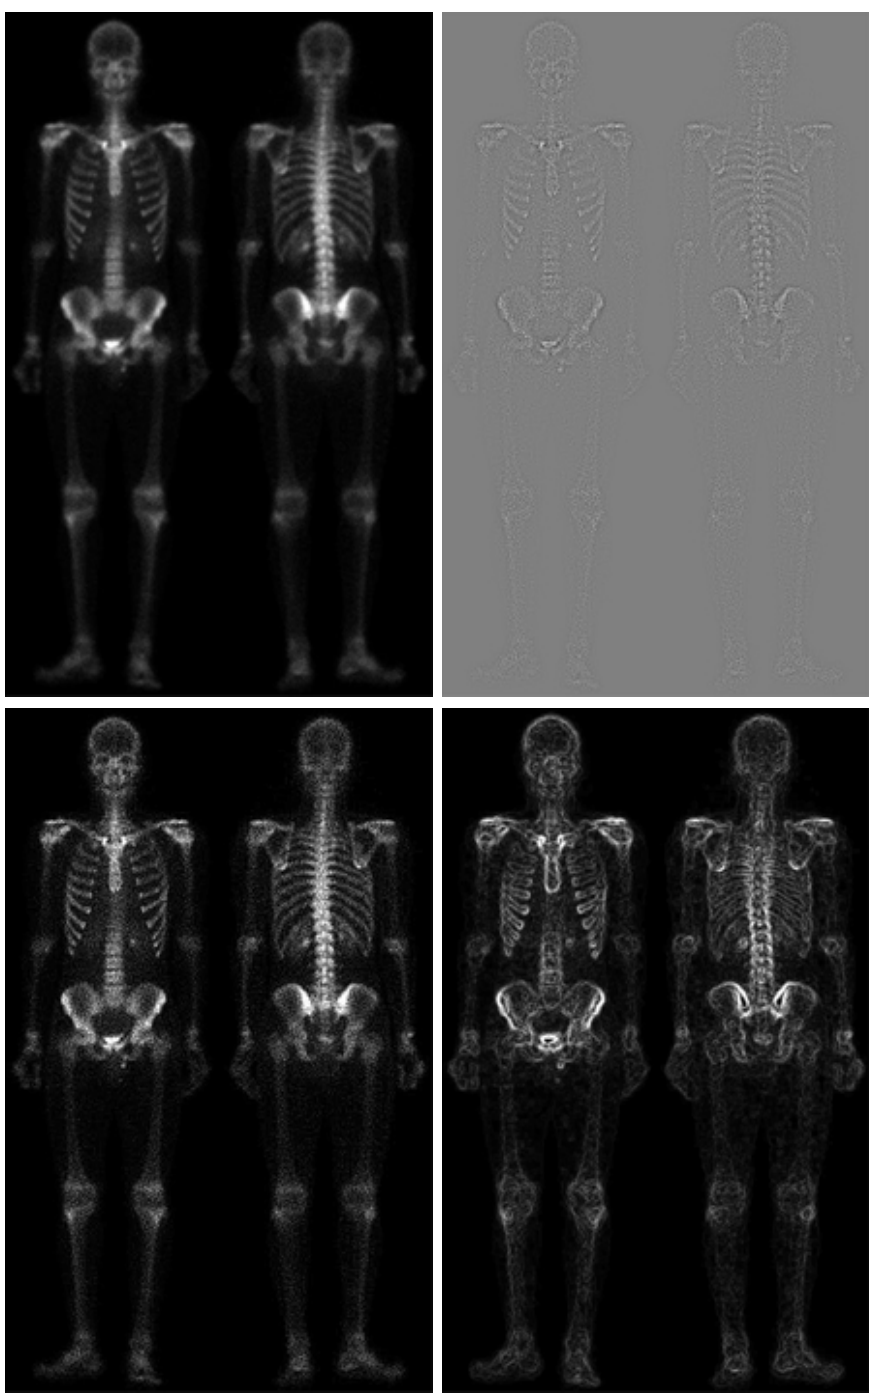
\includegraphics[scale=0.13]{images/Spatial12-ex1.png}
% \end{center}
% \end{frame}

% %----------

% \subsection{Image formation in the eye}

% \begin{frame}
%   \frametitle{Human Vision}
%   \framesubtitle{Image formation in the eye}
%   \begin{block}{Example}
%     \begin{figure}
%       \centering
%       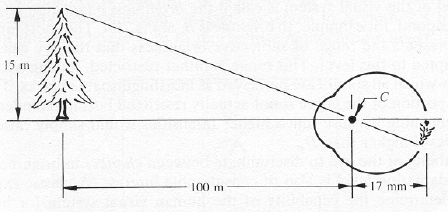
\includegraphics[width=.7\textwidth]{./images/form.png}
%     \end{figure}
%     \begin{itemize}\scriptsize
%     \item Focal length varies from 17 mm to 14 mm
%     \item Perception takes place by the relative excitation of light receptors.
%     \item The receptors transform this energy to electrical impulses
%     \end{itemize}
%   \end{block}
% \end{frame}

% \subsection{Brightness adaptation \& discrimination}

% \begin{frame}
%   \frametitle{Human Vision}
%   \framesubtitle{Brightness adaptation \& discrimination}
%   \begin{block}{Human visual system}
%     \begin{itemize}\scriptsize
%     \item The human vision system (HVS) can adapt to $10^{10}$ light intensity levels
%     \item Subjective brightness is a logarithmic function of the light intensity incident on the eye
%       \begin{figure}
%         \centering
%         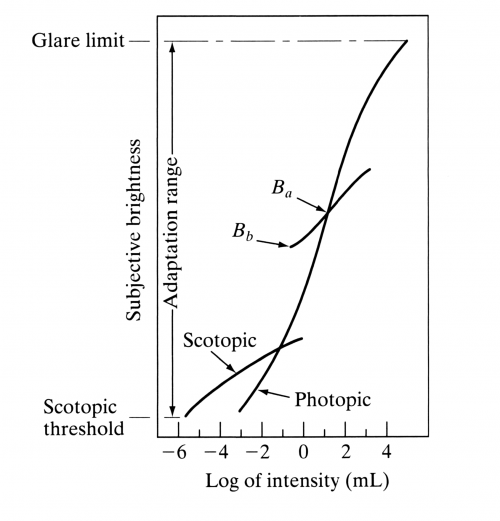
\includegraphics[height=.35\textheight]{./images/sb.png}
%       \end{figure}
%     \item The HVS cannot operate over such a range simultaneously
%     \item For a given set of conditions, the current sensitivity level is called \emph{brightness adaptation level}
%     \end{itemize}
%   \end{block}
% \end{frame}

% \begin{frame}
%   \frametitle{Human Vision}
%   \framesubtitle{Brightness adaptation \& discrimination}
%   \begin{block}{Human visual system}
%     \begin{itemize}\scriptsize
%     \item The eye also discriminates between changes in brightness at any specific adaption level
%     \item This is characterised by the Weber ratio
%     \end{itemize}
%     \begin{equation}
%       \frac{\Delta I_c}{I},
%     \end{equation}
%     {\scriptsize where $\Delta I_c$ is the increment of illumination discriminable 50 \% of the time and $I$ is the background illumination}
%   \end{block}
% \end{frame}

% \begin{frame}
%   \frametitle{Human Vision}
%   \framesubtitle{Brightness adaptation \& discrimination}
%   \begin{block}{Human visual system}
%     \begin{figure}
%       \centering
%       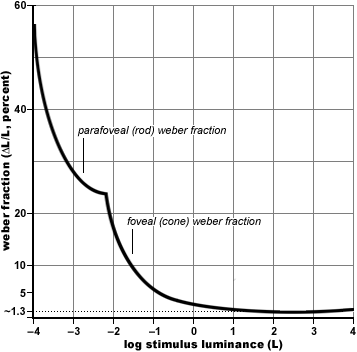
\includegraphics[height=.35\textheight]{./images/wr.png}
%     \end{figure}
%     \begin{itemize}\scriptsize
%     \item Small values of Weber ration mean good brightness discrimination and vice versa
%     \item At low levels of illumination brightness discrimination is poor (rods)
%     \item It improves significantly as background illumination increases (cones)
%     \item The typical observer can discern one to two dozen different intensity changes
%     \end{itemize}
%   \end{block}
% \end{frame}

% \begin{frame}
%   \frametitle{Human Vision}
%   \framesubtitle{Brightness adaptation \& discrimination}
%   \begin{block}{Human visual system}
%     \begin{itemize}\scriptsize
%     \item Overall intensity discrimination is broad due to different set of incremental changes to be detected at each new adaptation level
%     \item Perceived brightness is not a simple function of intensity: Mach band effect, simultaneously contrast, and optical effect
%     \end{itemize}
%   \end{block}
% \end{frame}

% \begin{frame}
%   \frametitle{Human Vision}
%   \framesubtitle{Brightness adaptation \& discrimination}
%     \only<1>{\begin{block}{Mach band effect}
%         \begin{figure}
%         \centering
%         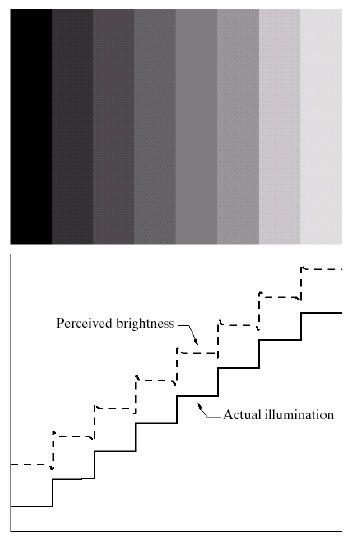
\includegraphics[height=.6\textheight]{./images/mach.png}
%       \end{figure}
%     \end{block}}
%   \only<2>{\begin{block}{Simultaneously contrast}
%         \begin{figure}
%         \centering
%         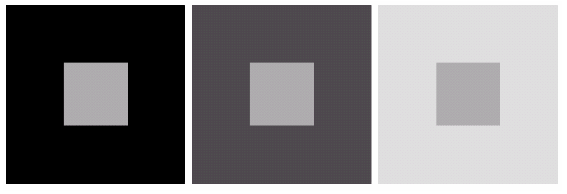
\includegraphics[width=.8\textwidth]{./images/sc.png}
%       \end{figure}
%     \end{block}}
%   \only<3>{\begin{block}{Optical effect}
%         \begin{figure}
%         \centering
%         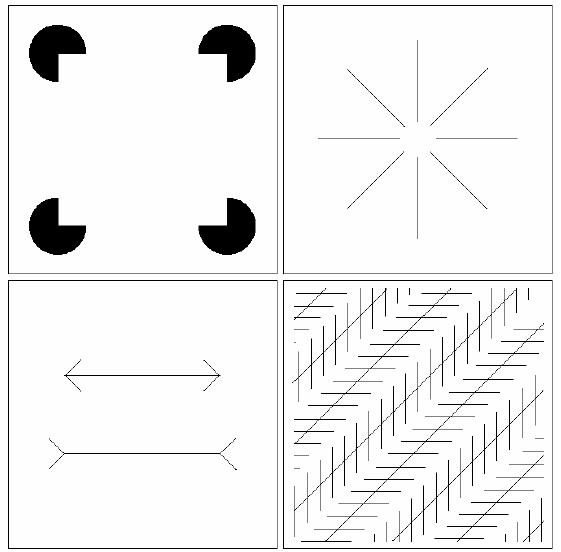
\includegraphics[height=.6\textheight]{./images/oe.png}
%       \end{figure}
%     \end{block}}
% \end{frame}

% \section{Digital Image}
% \subsection{Formation}

% \begin{frame}
%   \frametitle{Digital Image}
%   %\framesubtitle{}
%     \begin{block}{Digital image formation}
%         \begin{figure}
%         \centering
%         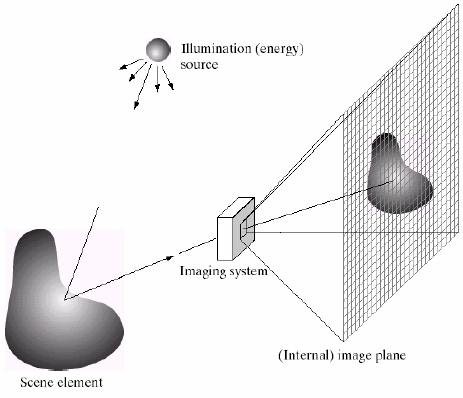
\includegraphics[height=.4\textheight]{./images/img_form.png}
%       \end{figure}
%       \begin{itemize}\scriptsize
%         \item $f(x,y)$: intensity or brightness of a pixel at a position $(x,y)$
%         \item $0 < f(x,y) < +\infty$
%       \end{itemize}
%     \end{block}
% \end{frame}

% \begin{frame}
%   \frametitle{Digital Image}
%   %\framesubtitle{}
%     \begin{block}{Digital image formation}
%         \begin{figure}
%         \centering
%         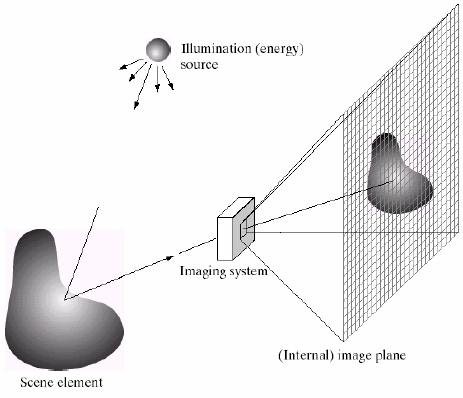
\includegraphics[height=.4\textheight]{./images/img_form.png}
%       \end{figure}
%       \begin{itemize}\scriptsize
%         \item<1-> $r(x,y)$: illumination --- $[0, +\infty[$
%         \item<2-> $i(x,y)$: reflectance --- $[0,1]$
%         \item<3-> $f(x,y) = r(x,y) i(x,y)$
%         \end{itemize}
%     \end{block}
% \end{frame}

% \begin{frame}
%   \frametitle{Digital Image}
%   %\framesubtitle{}
%     \begin{block}{Example of reflectance}
%       \begin{itemize}\scriptsize
%         \item Black velvet: 0.01
%         \item Snow: 0.93
%         \end{itemize}
%     \end{block}
%     \begin{block}{Example of illumination}
%       \begin{itemize}\scriptsize
%         \item Sunny day: 9000 foot-candles
%         \item Cloudy day: 1000 foot-candles
%         \item Full moon: 0.01 foot-candles
%         \end{itemize}
%     \end{block}
% \end{frame}

% \begin{frame}
%   \frametitle{Digital Image}
% %   %\framesubtitle{}
%     \begin{block}{In practise}
%       \begin{itemize}\scriptsize
%       \item $i(x,y)$ and $r(x,y)$ are bounded
%       \end{itemize}
%       {\scriptsize
%       \begin{eqnarray}
%         i_{\text{min}}(x_0, y_0) r_{\text{min}}(x_0, y_0) < & f(x_0, y_0) & < i_{\text{max}}(x_0, y_0) r_{\text{max}}(x_0, y_0) \ , \\
%         L_\text{min} < & f(x_0, y_0) & < L_\text{max} \ .
%       \end{eqnarray}}
%     \begin{itemize}
%       \item $[L_\text{min}, L_\text{max}] \approx [10, 1000]$ --- Shifted in $[0, L-1]$
%     \end{itemize}
%     \only<2>{
%     $\rightarrow$ What is the value for true white and black colors in an image?}
%     \end{block}
% \end{frame}

% \subsection{Sampling \& quantisation}

% \begin{frame}
%   \frametitle{Digital Image}
% %   %\framesubtitle{}
%     \only<1>{\begin{block}{Conversion from continuous to digital}
%       \begin{itemize}
%         \item $f(x,y)$ is a continuous function with regarding the coordinates and the amplitude
%         \item Image sampling to refer to spatial coordinates
%         \item Signal quantisation to digitise the amplitude 
%       \end{itemize}
%     \end{block}}
%   \only<2>{\begin{block}{Sampling}
%         \begin{figure}
%         \centering
%         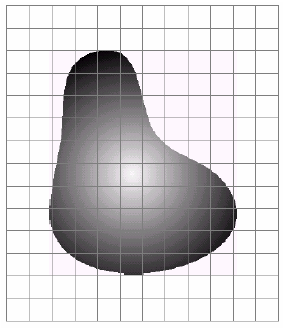
\includegraphics[height=.6\textheight]{./images/sampling.png}
%       \end{figure}
%     \end{block}}
%   \only<3>{\begin{block}{Quantisation}
%         \begin{figure}
%         \centering
%         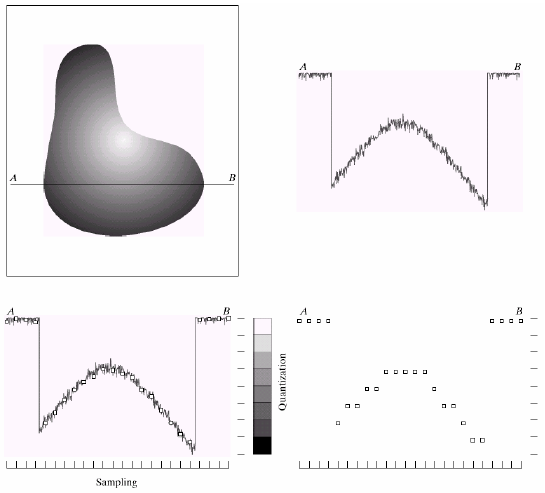
\includegraphics[height=.6\textheight]{./images/quantisation.png}
%       \end{figure}
%     \end{block}}
%   \only<4>{\begin{block}{Digital image}
%         \begin{figure}
%         \centering
%         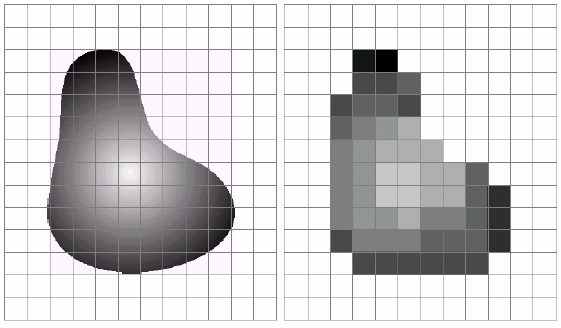
\includegraphics[height=.4\textheight]{./images/dig_img.png}
%       \end{figure}
%       \begin{itemize}\scriptsize
%         \item Check the appendix notebook
%       \end{itemize}
%     \end{block}}
% \end{frame}

% \begin{frame}
%   \frametitle{Digital Image}
% %   %\framesubtitle{}
%     \only<1>{\begin{block}{Coordinate system convention}
%         \begin{figure}
%         \centering
%         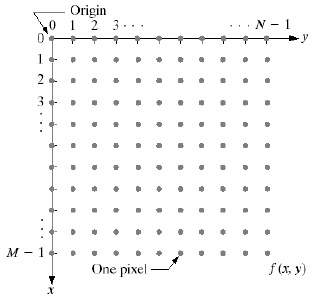
\includegraphics[height=.6\textheight]{./images/coo_img.png}
%       \end{figure}
%     \end{block}}
% \end{frame}

% \begin{frame}
%   \frametitle{Digital Image}
% %   %\framesubtitle{}
%     \only<1>{\begin{block}{Digitisation requirements}
%         \begin{itemize}\scriptsize
%           \item Set an height: $M$
%           \item Set an width: $N$
%           \item Set an intensity level: $L = 2^k$ and equally spaced
%           \item \emph{Dynamic range} : $\frac{L_{\text{min}}}{L_{\text{max}}}$
%         \end{itemize}
%         \begin{figure}
%         \centering
%         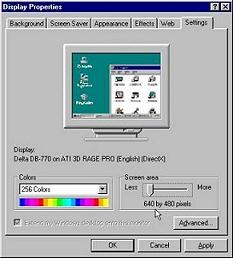
\includegraphics[height=.4\textheight]{./images/windows.jpg}
%       \end{figure}
%     \end{block}}
% \end{frame}

% \begin{frame}
%   \frametitle{Digital Image}
% %   %\framesubtitle{}
%     \only<1>{\begin{block}{Parameter variations}
%         \begin{figure}
%         \centering
%         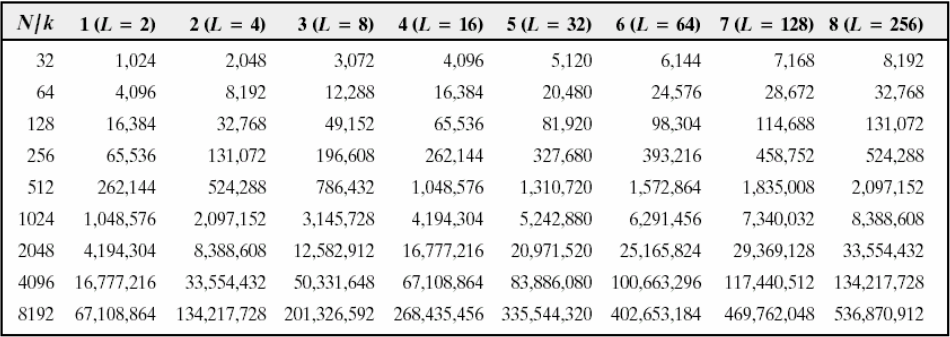
\includegraphics[width=.8\textwidth]{./images/storage.png}
%       \end{figure}
%       $\rightarrow$ What is the best values regarding the resolution and dynamic range parameters?
%       \begin{itemize}\scriptsize
%         \item Larger is better ...
%         \item ... storage and processing could be a problem
%       \end{itemize}
%     \end{block}}
% \end{frame}

% \begin{frame}
%   \frametitle{Digital Image}
% %   %\framesubtitle{}
%     \only<1>{\begin{block}{Isopreference curves}
%         \begin{figure}
%         \centering
%         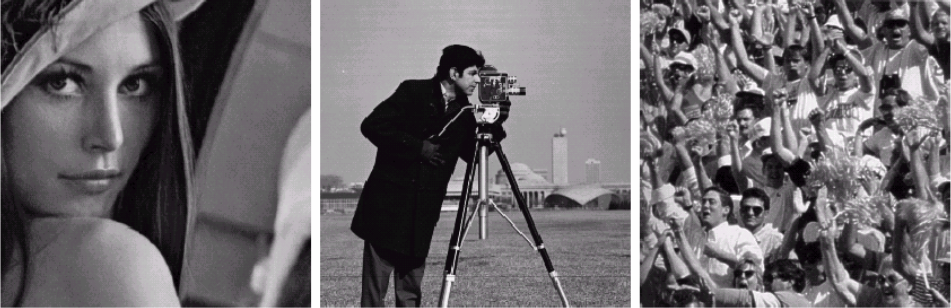
\includegraphics[width=.6\textwidth]{./images/iso1.png}
%       \end{figure}
%       \vspace{-.7cm}
%       \begin{figure}
%         \centering
%         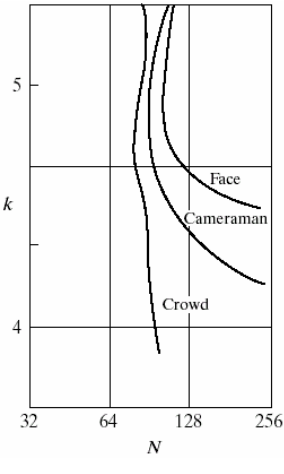
\includegraphics[height=.3\textheight]{./images/iso2.png}
%       \end{figure}
%     \end{block}}
% \end{frame}

% \begin{frame}
%   \frametitle{Digital Image}
% %   %\framesubtitle{}
%     \only<1->{\begin{block}{Non-uniform sampling and quantisation}
%         \begin{itemize}
%           \item<2-> Fine sampling in details region --- coarse sampling in smooth region
%           \item<3-> Few gray levels in details regions --- more in smooth region
%         \end{itemize}
%     \end{block}}
% \end{frame}

% \section{Pixel Relationships}

% \subsection{Neighbours}

% \begin{frame}
%   \frametitle{Pixel Relationships}
%   %   % \framesubtitle{}
%   \only<1->{\begin{block}{Neighours}\scriptsize
%       \begin{columns}
%         \begin{column}{.33\linewidth}
%           \begin{center}
%             \emph{4-neighbours} --- N\textsubscript{4}-p\\\vspace{.5cm}
%             \only<1>{\begin{tabular}{|c|c|c|c|c|}
%                 \hline
%                 0 & 1 & 1 & 1 & 0\\ \hline
%                 0 & 1 & 0 & 0 & 1\\ \hline
%                 0 & 0 & \cellcolor{azulunam!50}1 & 0 & 0\\ \hline
%                 1 & 0 & 1 & 1 & 0\\ \hline
%                 0 & 1 & 1 & 0 & 1\\ \hline
%               \end{tabular}}
%               \only<2->{\begin{tabular}{|c|c|c|c|c|}
%                 \hline
%                 0 & 1 & 1 & 1 & 0\\ \hline
%                 0 & 1 & \cellcolor{orounam!50}0 & 0 & 1\\ \hline
%                 0 & \cellcolor{orounam!50}0 & \cellcolor{azulunam!50}1 & \cellcolor{orounam!50}0 & 0\\ \hline
%                 1 & 0 & \cellcolor{orounam!50}1 & 1 & 0\\ \hline
%                 0 & 1 & 1 & 0 & 1\\ \hline
%               \end{tabular}}
%           \end{center}
%         \end{column}
%         \begin{column}{.33\linewidth}
%           \begin{center}
%           \emph{D-neighbours} --- N\textsubscript{D}-p\\\vspace{.5cm}
%             \only<1-2>{\begin{tabular}{|c|c|c|c|c|}
%                 \hline
%                 0 & 1 & 1 & 1 & 0\\ \hline
%                 0 & 1 & 0 & 0 & 1\\ \hline
%                 0 & 0 & \cellcolor{azulunam!50}1 & 0 & 0\\ \hline
%                 1 & 0 & 1 & 1 & 0\\ \hline
%                 0 & 1 & 1 & 0 & 1\\ \hline
%               \end{tabular}}
%               \only<3->{\begin{tabular}{|c|c|c|c|c|}
%                 \hline
%                 0 & 1 & 1 & 1 & 0\\ \hline
%                 0 & \cellcolor{orounam!50}1 & 0 & \cellcolor{orounam!50}0 & 1\\ \hline
%                 0 & 0 & \cellcolor{azulunam!50}1 & 0 & 0\\ \hline
%                 1 & \cellcolor{orounam!50}0 & 1 & \cellcolor{orounam!50}1 & 0\\ \hline
%                 0 & 1 & 1 & 0 & 1\\ \hline
%               \end{tabular}}
%           \end{center}
%         \end{column}
%         \begin{column}{.33\linewidth}
%           \begin{center}
%             \emph{8-neighbours} --- N\textsubscript{8}-p\\\vspace{.5cm}
%             \only<1-3>{\begin{tabular}{|c|c|c|c|c|}
%                 \hline
%                 0 & 1 & 1 & 1 & 0\\ \hline
%                 0 & 1 & 0 & 0 & 1\\ \hline
%                 0 & 0 & \cellcolor{azulunam!50}1 & 0 & 0\\ \hline
%                 1 & 0 & 1 & 1 & 0\\ \hline
%                 0 & 1 & 1 & 0 & 1\\ \hline
%               \end{tabular}}
%               \only<4>{\begin{tabular}{|c|c|c|c|c|}
%                 \hline
%                 0 & 1 & 1 & 1 & 0\\ \hline
%                 0 & \cellcolor{orounam!50}1 & \cellcolor{orounam!50}0 & \cellcolor{orounam!50}0 & 1\\ \hline
%                 0 & \cellcolor{orounam!50}0 & \cellcolor{azulunam!50}1 & \cellcolor{orounam!50}0 & 0\\ \hline
%                 1 & \cellcolor{orounam!50}0 & \cellcolor{orounam!50}1 & \cellcolor{orounam!50}1 & 0\\ \hline
%                 0 & 1 & 1 & 0 & 1\\ \hline
%               \end{tabular}}
%           \end{center}
%         \end{column}
%       \end{columns}
%     \end{block}}
% \end{frame}

% \subsection{Adjacency}

% \begin{frame}
%   \frametitle{Pixel Relationships}
%   %   % \framesubtitle{}
%   \begin{block}{Adjacency}\scriptsize
%       \begin{center}
%         \vspace{.1cm}
%         Let denotes $V=\{1\}$ defining the adjacency
%         \vspace{-.3cm}
%       \end{center}
%       \begin{columns}
%         \begin{column}{.33\linewidth}
%           \begin{center}
%             \emph{4-adjacency}\\\vspace{.5cm}
%             \only<1>{\begin{tabular}{|c|c|c|c|c|}
%                 \hline
%                 0 & 1 & 1 & 1 & 0\\ \hline
%                 0 & 1 & 0 & 0 & 1\\ \hline
%                 0 & 0 & \cellcolor{azulunam!50}1 & 0 & 0\\ \hline
%                 1 & 0 & 1 & 1 & 0\\ \hline
%                 0 & 1 & 1 & 0 & 1\\ \hline
%               \end{tabular}}
%             \only<2->{\begin{tabular}{|c|c|c|c|c|}
%                 \hline
%                 0 & 1 & 1 & 1 & 0\\ \hline
%                 0 & 1 & 0 & 0 & 1\\ \hline
%                 0 & 0 & \cellcolor{azulunam!50}1 & 0 & 0\\ \hline
%                 1 & 0 & \cellcolor{orounam!50}1 & 1 & 0\\ \hline
%                 0 & 1 & 1 & 0 & 1\\ \hline
%               \end{tabular}}
%           \end{center}
%         \end{column}
%         \begin{column}{.33\linewidth}
%           \begin{center}
%             \emph{8-adjacency}\\\vspace{.5cm}
%             \only<1-2>{\begin{tabular}{|c|c|c|c|c|}
%                 \hline
%                 0 & 1 & 1 & 1 & 0\\ \hline
%                 0 & 1 & 0 & 0 & 1\\ \hline
%                 0 & 0 & \cellcolor{azulunam!50}1 & 0 & 0\\ \hline
%                 1 & 0 & 1 & 1 & 0\\ \hline
%                 0 & 1 & 1 & 0 & 1\\ \hline
%               \end{tabular}}
%               \only<3->{\begin{tabular}{|c|c|c|c|c|}
%                 \hline
%                 0 & 1 & 1 & 1 & 0\\ \hline
%                 0 & \cellcolor{orounam!50}1 & 0 & 0 & 1\\ \hline
%                 0 & 0 & \cellcolor{azulunam!50}1 & 0 & 0\\ \hline
%                 1 & 0 & \cellcolor{orounam!50}1 & \cellcolor{orounam!50}1 & 0\\ \hline
%                 0 & 1 & 1 & 0 & 1\\ \hline
%               \end{tabular}}
%           \end{center}
%         \end{column}
%         \begin{column}{.33\linewidth}
%           \begin{center}
%             \emph{m-adjacency}\\\vspace{.5cm}
%             \only<1-3>{\begin{tabular}{|c|c|c|c|c|}
%                 \hline
%                 0 & 1 & 1 & 1 & 0\\ \hline
%                 0 & 1 & 0 & 0 & 1\\ \hline
%                 0 & 0 & \cellcolor{azulunam!50}1 & 0 & 0\\ \hline
%                 1 & 0 & 1 & 1 & 0\\ \hline
%                 0 & 1 & 1 & 0 & 1\\ \hline
%               \end{tabular}}
%               \only<4>{\begin{tabular}{|c|c|c|c|c|}
%                 \hline
%                 0 & 1 & 1 & 1 & 0\\ \hline
%                 0 & 1 & 0 & 0 & 1\\ \hline
%                 0 & 0 & \cellcolor{azulunam!50}1 & 0 & 0\\ \hline
%                 1 & 0 & \cellcolor{orounam!50}1 & 1 & 0\\ \hline
%                 0 & 1 & 1 & 0 & 1\\ \hline
%               \end{tabular}
%             $q \in N_4(p)$}
%           \only<5>{\begin{tabular}{|c|c|c|c|c|}
%                 \hline
%                 0 & 1 & 1 & 1 & 0\\ \hline
%                 0 & \cellcolor{orounam!50}1 & 0 & 0 & 1\\ \hline
%                 0 & 0 & \cellcolor{azulunam!50}1 & 0 & 0\\ \hline
%                 1 & 0 & 1 & \cellcolor{orounam!50}1 & 0\\ \hline
%                 0 & 1 & 1 & 0 & 1\\ \hline
%               \end{tabular}
%             $q \in N_D(p)$}
%           \only<6>{\begin{tabular}{|c|c|c|c|c|}
%                 \hline
%                 0 & 1 & 1 & 1 & 0\\ \hline
%                 0 & \cellcolor{orounam!50}1 & 0 & 0 & 1\\ \hline
%                 0 & 0 & \cellcolor{azulunam!50}1 & 0 & 0\\ \hline
%                 1 & 0 & 1 & 1 & 0\\ \hline
%                 0 & 1 & 1 & 0 & 1\\ \hline
%               \end{tabular}
%             $q \in N_D(p)$ AND $N_4(p) \cap N_4(q) \notin V$}
%           \only<7>{\begin{tabular}{|c|c|c|c|c|}
%                 \hline
%                 0 & 1 & 1 & 1 & 0\\ \hline
%                 0 & \cellcolor{orounam!50}1 & 0 & 0 & 1\\ \hline
%                 0 & 0 & \cellcolor{azulunam!50}1 & 0 & 0\\ \hline
%                 1 & 0 & \cellcolor{orounam!50}1 & 1 & 0\\ \hline
%                 0 & 1 & 1 & 0 & 1\\ \hline
%               \end{tabular}}
%           \end{center}
%         \end{column}
%       \end{columns}
%     \end{block}
% \end{frame}

% \subsection{Path}

% \begin{frame}
%   \frametitle{Pixel Relationships}
%   %   % \framesubtitle{}
%   \begin{block}{Path}\scriptsize
%     \begin{center}
%     \only<1>{\begin{tabular}{|c|c|c|c|c|}
%       \hline
%       0 & \cellcolor{azulunam!50}1 & 1 & 1 & 0\\ \hline
%       0 & 1 & 0 & 0 & 1\\ \hline
%       0 & 1 & 1 & 0 & 0\\ \hline
%       1 & 0 & 1 & 1 & 0\\ \hline
%       0 & 1 & 1 & 1 & \cellcolor{azulunam!50}1\\ \hline
%     \end{tabular}}
%   \only<2>{
%     4-path\\\vspace{.7cm}
%     \begin{tabular}{|c|c|c|c|c|}
%       \hline
%       0 & \cellcolor{azulunam!50}1 & 1 & 1 & 0\\ \hline
%       0 & \cellcolor{orounam!50}1 & 0 & 0 & 1\\ \hline
%       0 & \cellcolor{orounam!50}1 & \cellcolor{orounam!50}1 & 0 & 0\\ \hline
%       1 & 0 & \cellcolor{orounam!50}1 & 1 & 0\\ \hline
%       0 & 1 & \cellcolor{orounam!50}1 & \cellcolor{orounam!50}1 & \cellcolor{azulunam!50}1\\ \hline
%     \end{tabular}}
%   \only<3>{
%     8-path\\\vspace{.7cm}
%     \begin{tabular}{|c|c|c|c|c|}
%       \hline
%       0 & \cellcolor{azulunam!50}1 & 1 & 1 & 0\\ \hline
%       0 & \cellcolor{orounam!50}1 & 0 & 0 & 1\\ \hline
%       0 & 1 & \cellcolor{orounam!50}1 & 0 & 0\\ \hline
%       1 & 0 & 1 & \cellcolor{orounam!50}1 & 0\\ \hline
%       0 & 1 & 1 & 1 & \cellcolor{azulunam!50}1\\ \hline
%     \end{tabular}}
%     \only<4>{
%     m-path\\\vspace{.7cm}
%     \begin{tabular}{|c|c|c|c|c|}
%       \hline
%       0 & \cellcolor{azulunam!50}1 & 1 & 1 & 0\\ \hline
%       0 & \cellcolor{orounam!50}1 & 0 & 0 & 1\\ \hline
%       0 & \cellcolor{orounam!50}1 & \cellcolor{orounam!50}1 & 0 & 0\\ \hline
%       1 & 0 & \cellcolor{orounam!50}1 & 1 & 0\\ \hline
%       0 & 1 & \cellcolor{orounam!50}1 & \cellcolor{orounam!50}1 & \cellcolor{azulunam!50}1\\ \hline
%     \end{tabular}
%   \begin{itemize}
%     \item if $(x_{\text{init}}, y_{\text{init}}) = (x_{\text{end}}, y_{\text{end}}) \rightarrow$ closed path 
%   \end{itemize}}
%   \end{center}
%   \end{block}
% \end{frame}

% \subsection{Subset \& region}

% \begin{frame}
%   \frametitle{Pixel Relationships}
%   %   % \framesubtitle{}
%   \begin{block}{Subset}
%     \begin{itemize}
%     \item $p$ and $q$ are \emph{connected} in the subset $S$ if there is a path in with all the pixels belonging to $S$
%     \item For any pixel $p$ in $S$, the set of pixels in $S$ that are connected to p is a \emph{connected component} of $S$
%     \item If $S$ has only one connected component then $S$ is called a \emph{connected set}
%     \end{itemize}
%   \end{block}
%   \begin{block}{Region}
%     \begin{itemize}
%     \item $R$ is a subset of pixels: $R$ is a region if $R$ is a connected set
%     \item Region can be \emph{adjacent} or \emph{disjoint}
%     \end{itemize}
%   \end{block}
% \end{frame}

% \subsection{Distance measures}

% \begin{frame}
%   \frametitle{Pixel Relationships}
%   \framesubtitle{Distance measures}
%   \only<1>{\begin{block}{Definition}
%     For pixels $p,q,z$ with coordinates $(x,y)$, $(s,t)$, $(u,v)$, $D$ is a distance function or metric if:
%     \begin{itemize}
%     \item $D(p,q) \geq 0 \ (D(p,q)=0 \text{ iff } p=q)$
%     \item $D(p,q) = D(q,p)$ and
%     \item $D(p,z) \leq D(p,q) + D(q,z)$
%     \end{itemize}
%   \end{block}}
%   \only<2>{\begin{block}{Euclidean distance}
%     For pixels $p,q,z$ with coordinates $(x,y)$, $(s,t)$, $(u,v)$:
%     \begin{itemize}
%     \item  $D_e(p,q) = \sqrt{(x-s)^2 + (y-t)^2}$
%     \end{itemize}
%   \end{block}
%   \begin{block}{D\textsubscript{4} distance}
%     \begin{itemize}
%     \item  $D_4(p,q) = |x-s| + |y-t|$
%     \end{itemize}
%   \end{block}
%   \begin{block}{D\textsubscript{8} distance}
%     \begin{itemize}
%     \item  $D_8(p,q) = \text{max}(|x-s|, |y-t|)$
%     \end{itemize}
%   \end{block}
%   \begin{block}{D\textsubscript{m} distance}
%     \begin{itemize}
%     \item  Shortest $m$-path considering the $m$-adjacency
%     \end{itemize}
%   \end{block}}
% \end{frame}

\end{document}